\begin{figure}[htbp]
\centering
\begin{tikzpicture}[x=1cm,y=1cm]
\node[anchor=south west,inner sep=0] at (0,0) {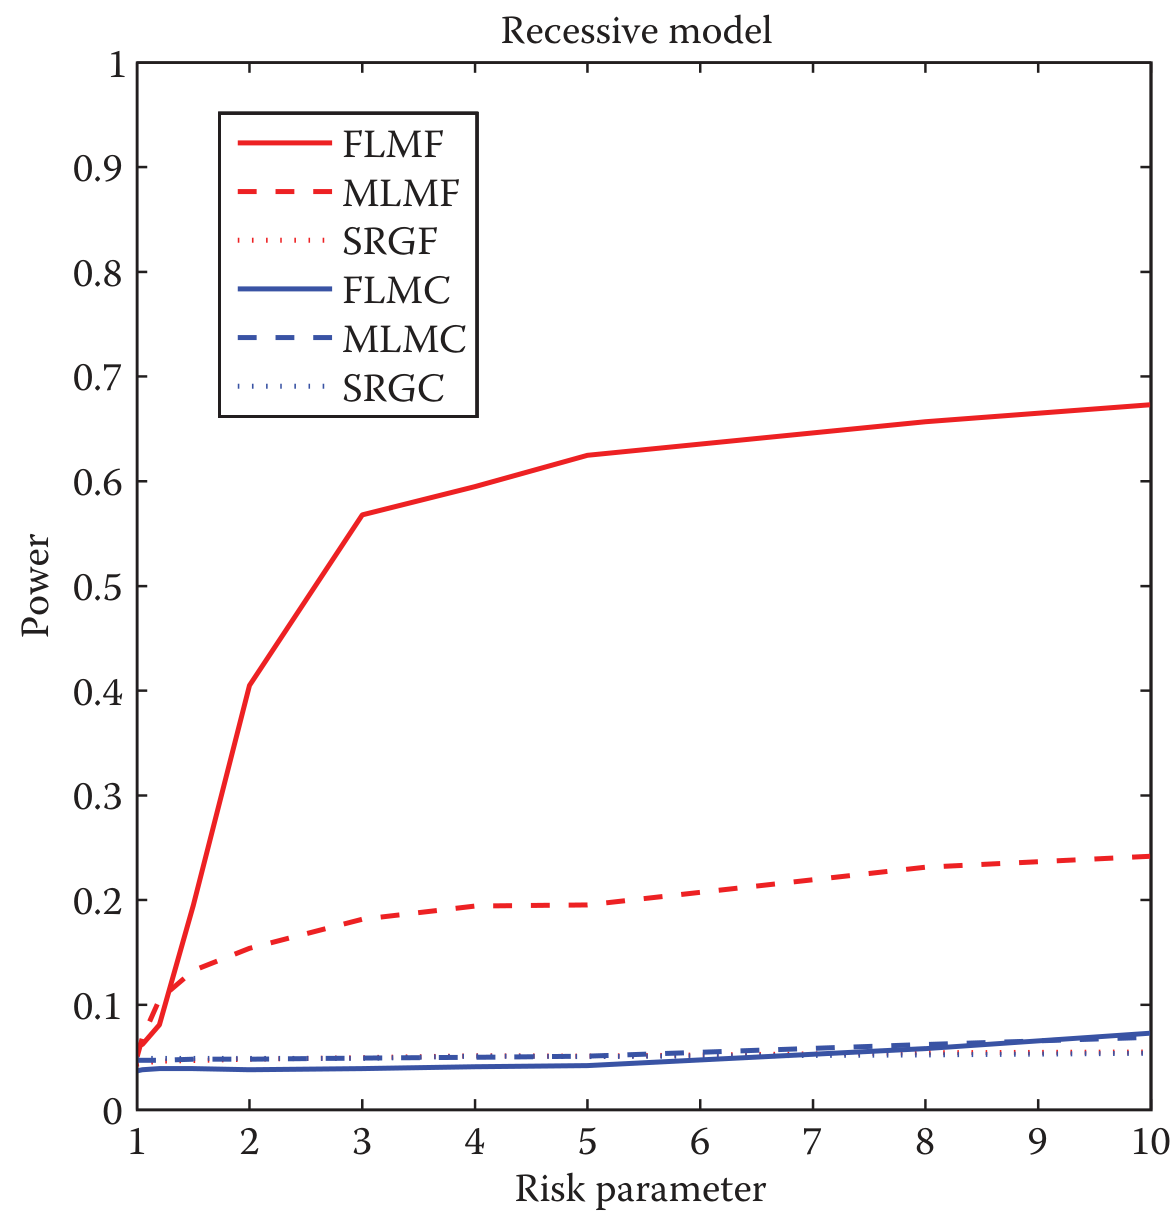
\includegraphics[width=13.0cm]{figures/ch03_fig18_data.png}};
\fill[white] (5.6853,0.0718) rectangle (8.5542,0.5718);
\node[font=\small,rotate=0,inner sep=0] at (7.1197,0.3218) {风险参数};
\fill[white] (0.1615,6.4322) rectangle (0.6726,7.6602);
\node[font=\small,rotate=90,inner sep=0] at (0.4171,7.0462) {统计功效};
\fill[white] (5.5303,12.9375) rectangle (8.6183,13.4375);
\node[font=\small,rotate=0,inner sep=0] at (7.0743,13.1875) {隐性模型};
\end{tikzpicture}
\origfig{18}{隐性模型下，六种模型的统计功效随风险参数的变化曲线。}
\label{fig:ch03-18}
\end{figure}
